%%%%%%%%%%%%%%%%%%%%%%%%%%%%%%%%%%%%%%%%%%%%%%%%
% E.Pinault-Bigeard - e.pinault-bigeard@upsti.fr
% http://s2i.pinault-bigeard.com
% CC BY-NC-SA 2.0 FR - http://creativecommons.org/licenses/by-nc-sa/2.0/fr/
%%%%%%%%%%%%%%%%%%%%%%%%%%%%%%%%%%%%%%%%%%%%%%%%
\documentclass[11pt]{article}
%%%%%%%%%%%%%%%%%%%%%%%%%%%%%%%%%%%%%%%%%%%%%%%%
% Package UPSTI_Document
%%%%%%%%%%%%%%%%%%%%%%%%%%%%%%%%%%%%%%%%%%%%%%%%
%%%%%%%%%%%%%%%%%%%%%%%%%%%%%%%%%%%%%%%%%%%%%%%%
% Package UPSTI_Document
%%%%%%%%%%%%%%%%%%%%%%%%%%%%%%%%%%%%%%%%%%%%%%%%
\usepackage{subcaption}
\usepackage[usenames, svgnames, dvipsnames]{xcolor}
\usepackage{UPSTI_Document}
\usepackage{pgfplots}
\usepackage{import}
\definecolor{darkspringgreen}{rgb}{0.09, 0.45, 0.27}

\newcommandx*{\dessinRepereFigGeo}[5][1=\vx{},2=\vy{},3=\vz{},4=,5=0]
	{
		\draw [->,very thick] (0,0) -- (1,0) ;
		\draw [->,very thick] (0,0) -- (0,1) ;
    \fill[white] (0,0) circle (0.13);
    \draw [->,very thick] (0,0) circle (0.13);
    \ifnumequal{#5}{0} {% z vers nous
      \fill[black] (0,0) circle (0.03);
      \draw [->,thick] (0,0) circle (0.04);
    }{% z vers la feuille
  		\begin{scope} [rotate=45]
  			\draw [-,thick] (0,-0.12) -- (0,0.12) ;
  			\draw [-,thick] (-0.12,0) -- (0.12,0) ;
  		\end{scope}
    }
		\draw [anchor=north west] (1.1,0) node {${#1}$};
		\draw [anchor=south west] (0,1.1) node {${#2}$};
		\draw [anchor=north east] (-0.1,0) node {${#3}$};
		\draw [anchor=north west] (-0.1,-0.1) node {${#4}$};
	}

	\usepackage{array}
	\newcolumntype{L}[1]{>{\raggedright\let\newline\\\arraybackslash\hspace{0pt}}m{#1}}
	\newcolumntype{C}[1]{>{\centering\let\newline\\\arraybackslash\hspace{0pt}}m{#1}}
	\newcolumntype{R}[1]{>{\raggedleft\let\newline\\\arraybackslash\hspace{0pt}}m{#1}}

	\usepackage{pifont}% http://ctan.org/pkg/pifont
\newcommand{\cmark}{\color{green}\ding{51}}%
\newcommand{\xmark}{\color{red}\ding{55}}%
\newcommand{\fmark}{\ding{229}}%
\newcommand{\itemc}{\item[\cmark]}%
\newcommand{\itemx}{\item[\xmark]}%
\newcommand{\itemf}{\item[\fmark]}%


\usetikzlibrary[circuits.plc.ladder]            %     
\newlength{\ladderskip}\setlength{\ladderskip}{5\tikzcircuitssizeunit}%5\tikzcircuitssizeunit    = 355pt
\newlength{\ladderrungsep}
\setlength{\ladderrungsep}{.2\ladderskip}
\def\ladderrungend#1{\pgftransformyshift{-#1\ladderskip-\ladderrungsep}}

%---------------------------------%
% Paramètres du package
%---------------------------------%

% Version du document (pour la compilation)
% 1: Document prof
% 2: Document élève
% 3: Document à publier
\newcommand{\UPSTIidVersionDocument}{2}


% Classe
% 1: PTSI				6: PSI*			11: TSI2		16: Spé
% 2: PT	(par défaut)	7: MPSI			12: ATS
% 3: PT*				8: MP			13: PC
% 4: PCSI				9: MP*			14: PC*
% 5: PSI				10: TSI1		15: Sup
%\newcommand{\UPSTIidClasse}{2}



% Matière
% 1: S2I (par défaut)    2: IPT     3: TIPE
% 6: Vie au lycée
\newcommand{\UPSTIvariante}{5}
\newcommand{\UPSTIidMatiere}{0}
\newcommand{\UPSTIintituleMatiere}{Automatique}
\newcommand{\UPSTIsigleMatiere}{Autom}
% Type de document
% 0: Custom*				7: Fiche Métho de			14: Document Réponses
% 1: Cours (par défaut)		8: Fiche Synthèse    		15: Programme de colle
% 2: TD     				9: Formulaire
% 3: TP						10: Memo
% 4: Colle					11: Dossier Technique
% 5: DS						12: Dossier Ressource
% 6: DM						13: Concours Blanc
% * Si on met la valeur 0, il faut décommenter la ligne suivante:
%\newcommand{\UPSTItypeDocument}{Custom}
\newcommand{\UPSTIidTypeDocument}{1}

% Titre dans l'en-tête


% Titre dans l'en-tête

\newcommand{\UPSTIvariante}{5}

\newcommand{\UPSTItitreEnTete}{Automatisme industriel}
%\newcommand{\UPSTItitreEnTetePages}{}
\newcommand{\UPSTIsousTitreEnTete}{Introduction aux API}


% Titre
%\newcommand{\UPSTItitrePreambule}{Automatisme industriel}
\newcommand{\UPSTItitre}{La programmation d'un Automate Industriel}

% Durée de l'activité (pour DS, DM et TP)
\newcommand{\UPSTIduree}{3h30}

% Note de bas de première page
%\newcommand{\UPSTInoteBasDePremierePage}{Geoffrey Vaquette}
% Numéro (ajoute " n°1" après DS ou DM)
\newcommand{\UPSTInumero}{2}

% Numéro chapitre
%\newcommand{\UPSTInumeroChapitre}{1}

% En-tête customisé
%\newcommand{\UPSTIenTetePrincipalCustom}{UPSTIenTetePrincipalCustom}

% Message sous le titre
%\newcommand{\UPSTImessage}{Message sous le titre}


% Référence au programme
%\newcommand{\UPSTIprogramme}{\EPBComp \EPBCompP{B1-02}, \EPBCompP{B2-49}, \EPBCompS{B2-50}, \EPBCompS{B2-51}, \EPBCompP{C1-07}, \EPBCompP{C1-08}}

% Si l'auteur n'est pas l'auteur par défaut
%\renewcommand{\UPSTIauteur}{WWOOOOOOWW}

% Si le document est réalisé au nom de l'équipe
%\newcommand{\UPSTIdocumentCollegial}{1}

% Source
\newcommand{\UPSTIsource}{G. Vaquette, H. Discours}

% Version du document
\newcommand{\UPSTInumeroVersion}{1.0}

%-----------------------------------------------
\UPSTIcompileVars		% "Compile" les variables
%%%%%%%%%%%%%%%%%%%%%%%%%%%%%%%%%%%%%%%%%%%%%%%%


%%%%%%%%%%%%%%%%%%%%%%%%%%%%%%%%%%%%%%%%%%%%%%%%
% Début du document
%%%%%%%%%%%%%%%%%%%%%%%%%%%%%%%%%%%%%%%%%%%%%%%%
\begin{document}
\UPSTIbuildPage

%\UPSTIobjectif{Durant cette activité, nous allons analyser une trame pour l'envoi d'informations sur une étiquette.}

\tableofcontents

% \begin{figure}[bht]
%     \centering
%             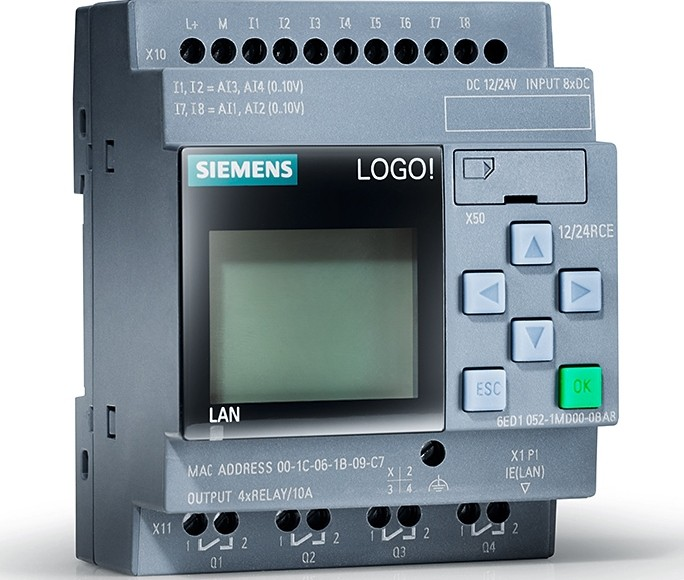
\includegraphics[width=.6\textwidth, height=.2\textheight,keepaspectratio]{images/logo-v8-siemens}
%             \caption{Automate Monobloc : Siemens LOGO}
%             \label{fig:logo}
% \end{figure}
\pagebreak
\section{Présentation de l'automate \textbf{LOGO} Siemens}



L'automate LOGO est un automate Monobloc de la marque Siemens. 
\textit{Monobloc} signifie qu'il contient nativement des entrées et des sorties directement sur le bloc de la CPU. 



\begin{UPSTIactivite}
    Un automate LOGO a été mis à votre disposition. Il est composé notamment de : 
    \begin{itemize}
        \item Deux bornes d'alimentation
        \item Huit entrées logiques
        \item Quatre sorties logiques à relais
        \item Une prise RJ45 pour se relier au réseau
        \item Une IHM composée de
        \begin{itemize}
            \item Un écran LCD
            \item Cinq boutons 
        \end{itemize}
    \end{itemize}

    \UPSTIquestion{Identifier les différents éléments composant la base du LOGO sur l'image suivante.}
    \UPSTIquestion{A l'aide de la documentation et de la référence sur le module, identifier et donner les caractéristiques des modules d'extension présents sur la maquette}

    \begin{center}
        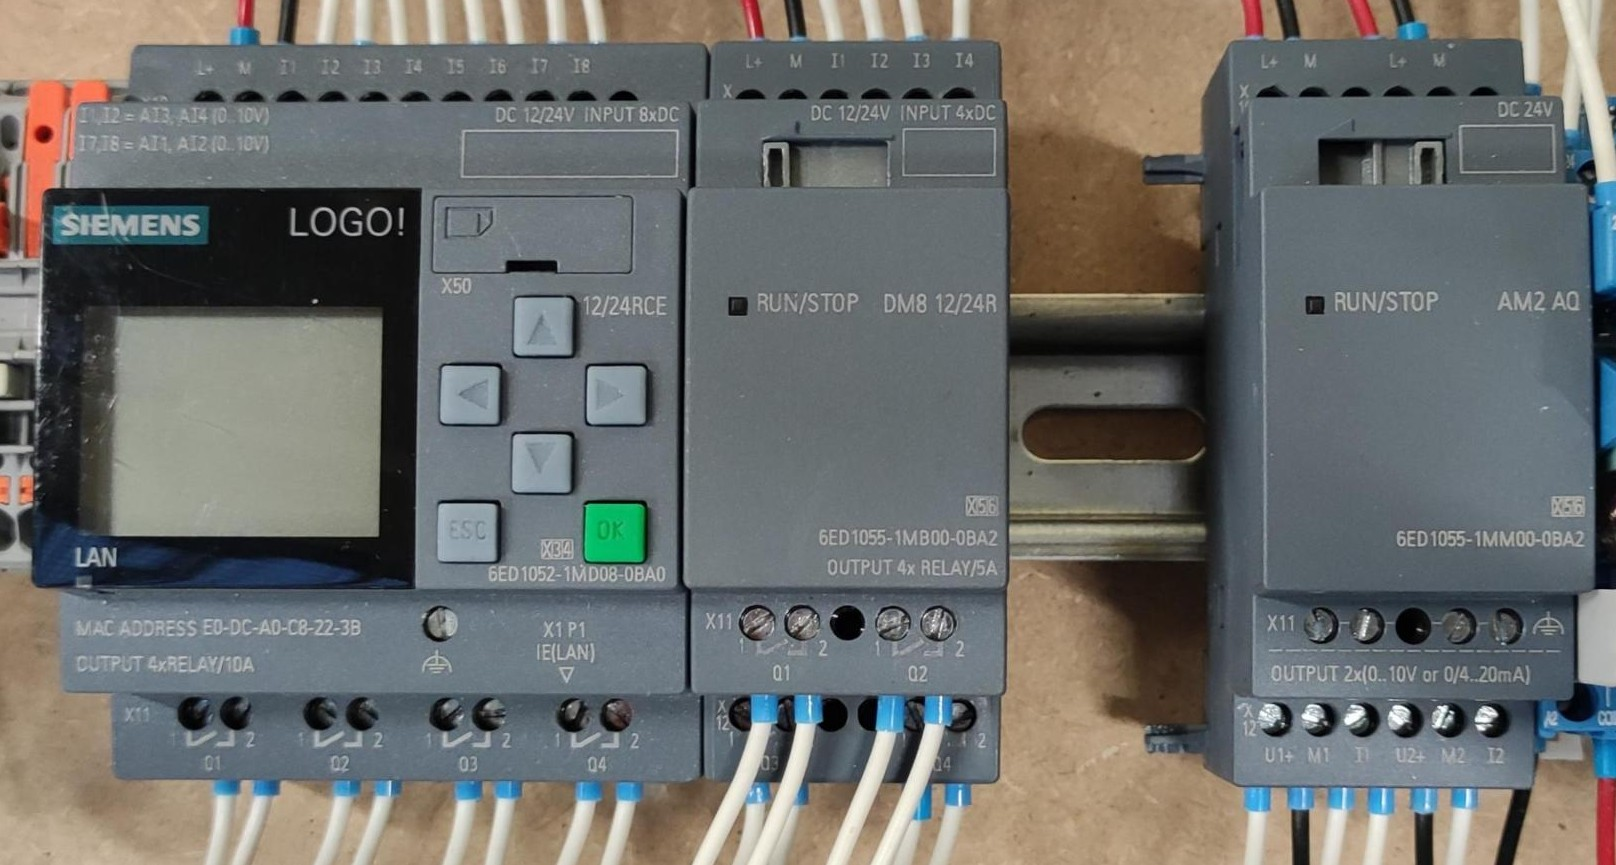
\includegraphics[width=.6\textwidth, height=.35\textheight,keepaspectratio]{images/maquette_logo.jpg}
    \end{center}

\end{UPSTIactivite}



\section{Prise en main du LOGO}
%\subsection{Tutoriel vidéo}
\begin{UPSTIactivite}
    Cette activité permet la prise en main d'un automate LOGO. 

    Tout d'abord, visionner et suivre la \href{https://www.youtube.com/watch?v=ATcv0Dwm8ok}{vidéo} \url{https://www.youtube.com/watch?v=ATcv0Dwm8ok}.
    
    En utilisant des boutons poussoir au lieu des interrupteurs, réaliser le câblage proposé dans la vidéo et faire valider par l'enseignant. 
\end{UPSTIactivite}
\pagebreak

Le langage LADDER fut conçu dans les années 1970 pour faire passer les électrotechniciens de la saisie de schémas électriques de systèmes à relais  à la programmation.
Il est donc simple et proche de la description de schémas électriques.
On le réserve à la description de fonctions combinatoires ou à des calculs simples.

Une ligne d'un programme LADDER est appelée réseau.

Un réseau est composé de contacts, de bobine et/ou de blocs.

\subsection{Réseaux LADDER simples}

\subsubsection{Les contacts}

Les contacts représentent des entrées logiques (TOR).

\UPSTIaRetenir{Il existe deux types de contacts :
\begin{description}
  \item [$\begin{array}{l}\begin{tikzpicture}[circuit plc ladder,thick,x=\ladderskip,y=\ladderskip]
  \draw(0,0) to [contact NO={info={a}}] ++ (1,0);
\end{tikzpicture}
 \end{array}$] \textbf{Contact normalement ouvert} :
  actif lorsque la variable associée est à l'état 1.
  \begin{itemize}
    \item [$\Rightarrow$] Il représente donc la variable $a$
  \end{itemize}
  \item [$\begin{array}{l}\begin{tikzpicture}[circuit plc ladder,thick,x=\ladderskip,y=\ladderskip]
  \draw(0,0) to [contact NC={info={a}}] ++ (1,0);
\end{tikzpicture}
 \end{array}$]  \textbf{Contact normalement fermé } actif lorsque la variable associée est à l'état 0.
  \begin{itemize}
    \item [$\Rightarrow$] Il représente donc la variable $\overline{a}$
  \end{itemize}
\end{description}
}

\subsubsection{Les bobines}

Les bobines représentent les sorties logiques (TOR) de l'API.

\UPSTIaRetenir{Une sortie S de l'automate est active lorsque la bobine associée $\begin{array}{l}\begin{tikzpicture}[circuit plc ladder,thick,x=\ladderskip,y=\ladderskip]
  \draw(0,0) to [coil={info={S}}] ++ (1,0);
\end{tikzpicture}
\end{array}$ est active.}


\subsubsection{Réseaux de base}

La traduction en réseau LADDER de l'équation $S = a$ est donc représentée sur la figure \ref{fig:ladAtoS}. L'équation en réseau LADDER de l'équation $S = \overline{a}$ est représentée sur la figure~\ref{fig:ladABartoS}

\begin{figure}[ht]
  \begin{subfigure}[b]{.49\textwidth}
  \centering
    \begin{tikzpicture}[circuit plc ladder, thick, x=\ladderskip, y=\ladderskip]
  \draw(0,0) to [contact NO={info={a}}] ++ (1,0) -- ++(1,0)
    to [coil={info={Sortie}}] + (1,0) coordinate(laddertopright);
    \ladderrungend{1.2}
    \draw let \p1=(laddertopright) in
    (0,   \y1+0.7\ladderskip) -- (0,    \ladderskip)
    (\x1, \y1+0.7\ladderskip) -- (\x1,  \ladderskip);
\end{tikzpicture}

    \caption{$S = a$}
    \label{fig:ladAtoS}
  \end{subfigure}
  %
  \begin{subfigure}[b]{.49\textwidth}
  \centering
    \begin{tikzpicture}[circuit plc ladder, thick, x=\ladderskip, y=\ladderskip]
  \draw(0,0) to [contact NC={info={a}}] ++ (1,0) -- ++(1,0)
    to [coil={info={Sortie}}] + (1,0) coordinate(laddertopright);
    \ladderrungend{1.2}
    \draw let \p1=(laddertopright) in
    (0,   \y1+0.7\ladderskip) -- (0,    \ladderskip)
    (\x1, \y1+0.7\ladderskip) -- (\x1,  \ladderskip);
\end{tikzpicture}

    \caption{$S = \overline{a}$}
    \label{fig:ladABartoS}
  \end{subfigure}

  \caption{Réseaux LADDER de base}
\end{figure}

Comme dans un circuit électrique, il est possible de programmer des équation combinatoires en langage LADDER. Les fonctions \textbf{ET} et \textbf{OU} sont représentée sur la figure~\ref{fig:equaLogiques}

\begin{figure}[ht]
  \begin{subfigure}[b]{.49\textwidth}
    \centering
    \begin{tikzpicture}[circuit plc ladder, thick, x=\ladderskip, y=\ladderskip]
  \draw(0,0) to [contact NO={info={a}}] ++ (1,0)
    to [contact NO={info={b}}] ++ (1,0) -- ++(1,0)
    to [coil={info={Sortie}}] + (1,0) coordinate(laddertopright);
    \ladderrungend{1.2}
    \draw let \p1=(laddertopright) in
    (0,   \y1+0.7\ladderskip) -- (0,    \ladderskip)
    (\x1, \y1+0.7\ladderskip) -- (\x1,  \ladderskip);
\end{tikzpicture}

    \caption{$S = a \text{ ET } b$}
    \label{fig:aETb}
  \end{subfigure}
  %
  \begin{subfigure}[b]{.49\textwidth}
    \centering 
    \begin{tikzpicture}[circuit plc ladder,thick,x=\ladderskip,y=\ladderskip]
  \draw(0,0) to [contact NO={info={a}}] ++ (1,0) coordinate(laddercoil) -- ++(2,0) to [coil={info={Sortie}}] ++ (1,0) coordinate(laddertopright);
  \draw(0,-1) to [contact NO={info={b}}] ++ (1,0) -- (laddercoil);

  \ladderrungend{2}
  \draw let \p1=(laddertopright) in
  (0,   \y1+0.7\ladderskip) -- (0,    \ladderskip)
  (\x1, \y1+0.7\ladderskip) -- (\x1,  \ladderskip);
\end{tikzpicture}

    \caption{$S = a \text{ OU } b$}
    \label{fig:aOUb}
  \end{subfigure}
  \caption{Equations logiques simples}
  \label{fig:equaLogiques}
\end{figure}

\begin{UPSTIactivite}
    \UPSTIquestion{Dessinez le réseau LADDER de l'équation $S = a + \overline{b}$}

    \UPSTIlignesACompleter[2]{\begin{center}
      \input{ladder_diagrams/ladCircuitaOubBar.tikz}
    \end{center}}

    \UPSTIquestion{Dessinez le réseau LADDER de l'équation $S = \overline{a} \cdot \overline{b}$}

    \UPSTIlignesACompleter[2]{\begin{center}
      \input{ladder_diagrams/ladABarETBBar.tikz}
    \end{center}}

    \UPSTIquestion{Dessinez le réseau LADDER de l'équation $S = (a + b) \cdot \overline{b} \cdot c $}

    \UPSTIlignesACompleter[2]{\begin{center}
      \input{ladder_diagrams/lad_AOuB_ET_BBar_ET_C.tikz}
    \end{center}}


\end{UPSTIactivite}


\pagebreak
\subsection{Application LADDER}
\begin{UPSTIactivite}[][LADDER]
    Soit le schéma suivant : 

    \begin{center}
        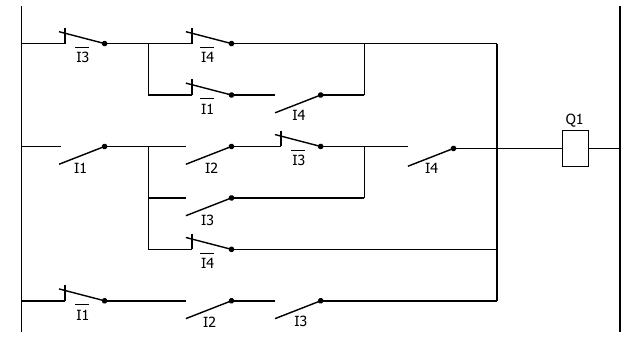
\includegraphics[width=.8\textwidth]{images/TP01_Ex01_cablage}
    \end{center}

    \begin{enumerate}
        \item Saisir ce schéma en LADDER dans LogoSoft
        \item A l'aide du simulateur, faire varier les entrées pour établir la table de vérité de la sortie Q1
        \item Transformer ce schéma en logigramme à l'aide de l'icone 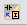
\includegraphics[height=\fontcharht\font`\B]{images/logoSoft_laderToSchema.png} et déterminer l'équation logique de la sortie Q1 
    \end{enumerate}
\end{UPSTIactivite}

\section{Exercice : Contrôle dimensionnel de pièces mécaniques}

\begin{figure}[ht]
    \centering
    \begin{subfigure}{0.49\textwidth}
        \centering
        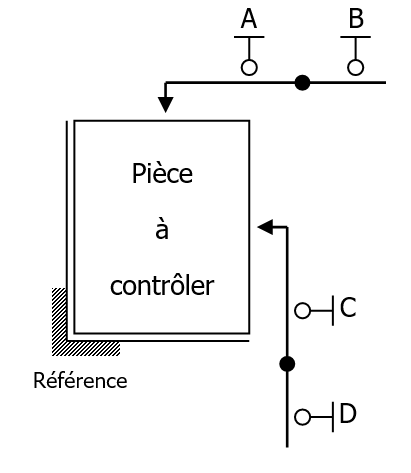
\includegraphics[width=\textwidth, height=.25\textheight, keepaspectratio]{images/TP01_Ex02_palpeur01}
        \caption{Pièce OK}
    \end{subfigure}
    \begin{subfigure}{0.49\textwidth}
        \centering
        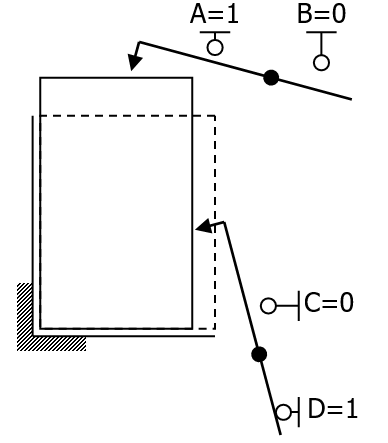
\includegraphics[width=\textwidth, height=.25\textheight, keepaspectratio]{images/TP01_Ex02_palpeur02}
        \caption{Pièce à rejeter}
    \end{subfigure}
    \caption{Palpeurs d'une pièce mécanique}
    \label{fig:palpeurs}
\end{figure}

Soit un système de contrôle dimensionnel de pièces mécaniques utilisant quatre capteurs A, B, C et D assoicés à deux palpeurs comme sur la Figure~\ref{fig:palpeurs}

Comme indiqué sur la Figure, les 4 capteurs sont inactifs pour une pièce de taille correcte. 

Le système de contrôle doit délivrer trois informations : 
\begin{description}
    \item[OK] lorsque la pièce est de taille correcte
    \item[Usinage] lorsque la pièce est trop grande sans qu'un côté soit trop petit
    \item[REJET] lorsque la pièce a au moins un côté trop petit  
\end{description}

\begin{table}[ht]
    \centering
    \begin{tabular}[]{c|c}
        Capteur & Entrée \\\hline
        A       &  I1\\
        B       &  I2\\
        C       &  I3\\
        D       &  I4\\
    \end{tabular}
    \caption{Correspondance Capteur - Entrée de l'automate}
\end{table}


\begin{UPSTIactivite}
    \UPSTIquestion{A l'aide de la Figure~\ref{fig:palpeurs}, donner les capteurs actifs lorsque la pièce est \begin{itemize}
        \item Trop haute
        \item Trop large
        \item Pas suffisamment hautre
        \item Pas suffisamment large
    \end{itemize}}

    %\UPSTIquestion{Etablir la table de vérité du système}
    \UPSTIquestion{Donner les équations de chaque sortie}
    \UPSTIquestion{Programmer le fonctionnement dans le langage de votre choix.}

    Les message seront affichés sur l'écran du LOGO : 
    \begin{itemize}
        \item OK sur fond BLANC
        \item USINAGE sur fond ORANGE
        \item REJET sur fond ROUGE 
    \end{itemize}
    \centering
    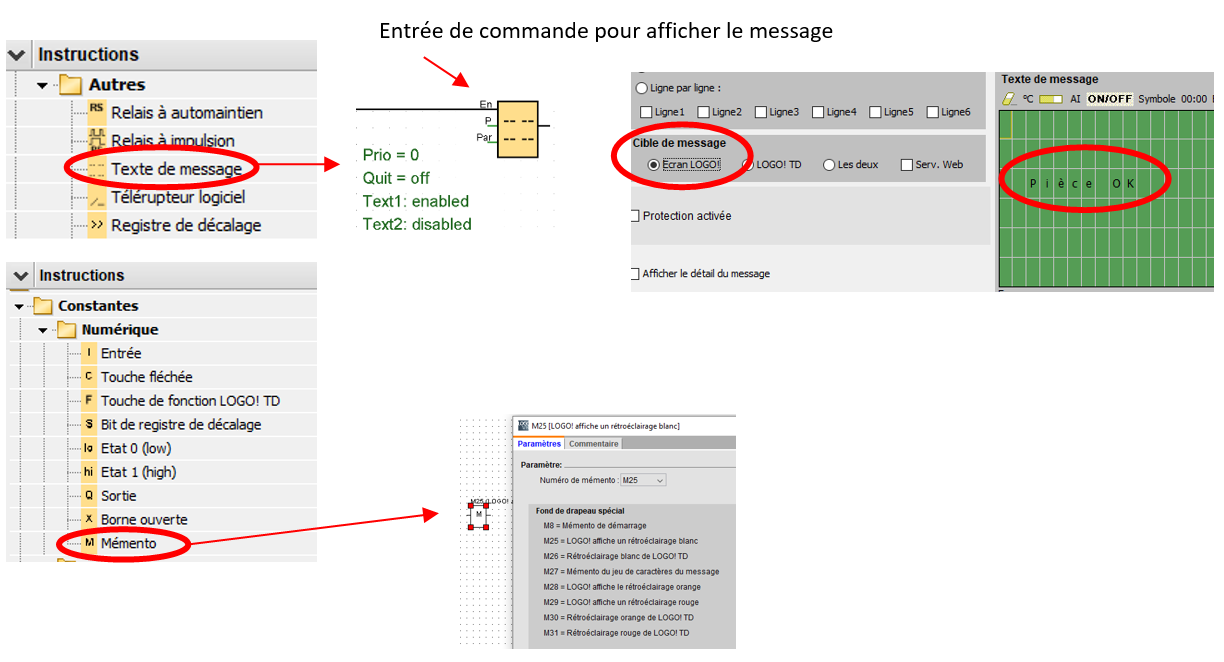
\includegraphics[width=.8\textwidth]{images/TP01_couleur_ecran.png}





\end{UPSTIactivite}
\pagebreak
\appendix
\section{Documentation LOGO et extensions}
\label{sec:Documentation}
\subsection{Modules de base}
\begin{table}[h!]
    \centering
    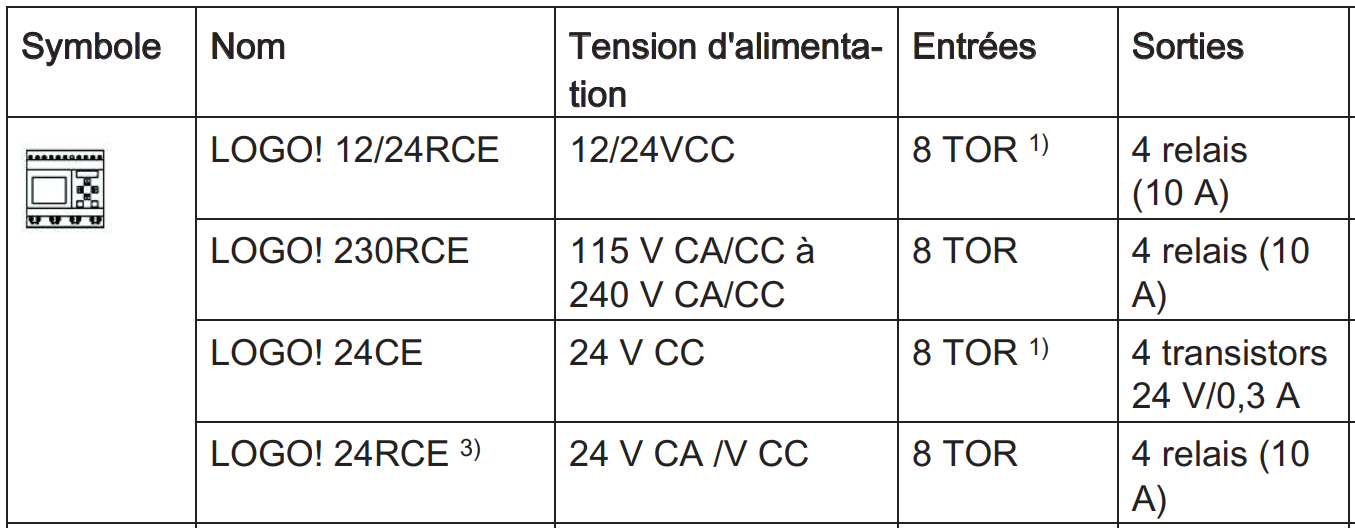
\includegraphics[width=\textwidth,height=.4\textheight,keepaspectratio]{images/doc_base_logo}
    \caption{Caractéristiques du module de base}
\end{table}

\subsection{Modules d'extension}
\begin{table}[h!]
    \centering
    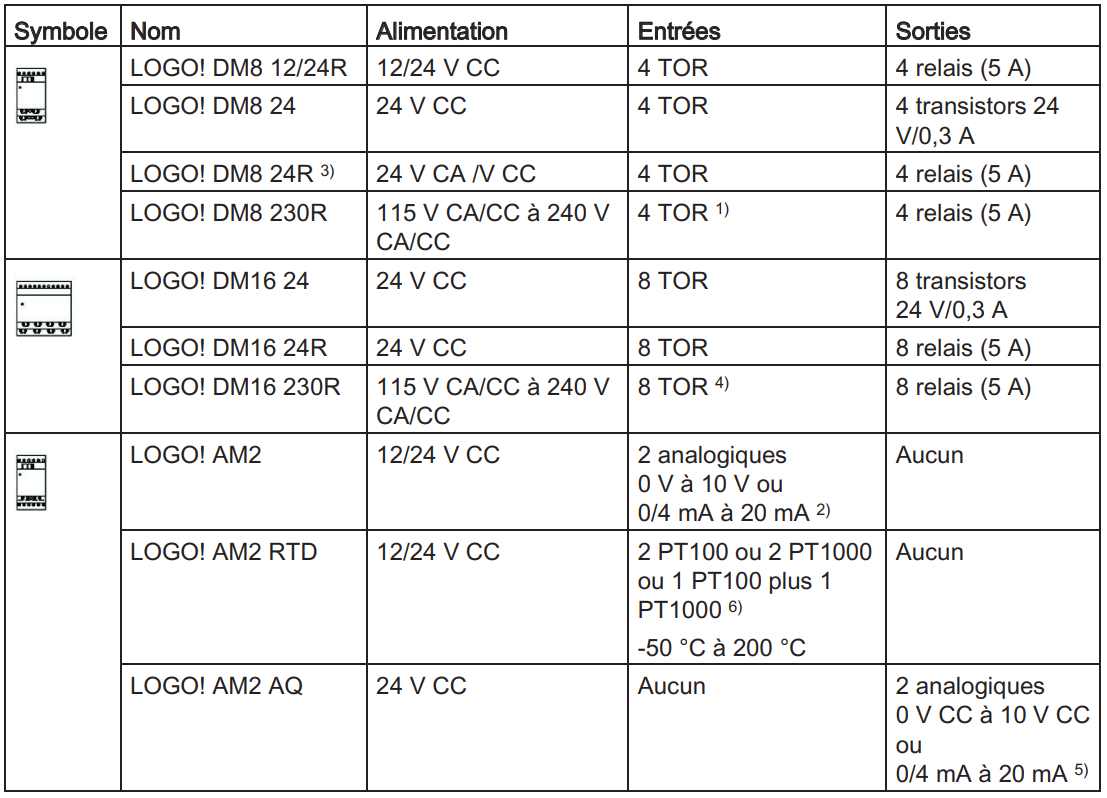
\includegraphics[width=\textwidth,height=.4\textheight,keepaspectratio]{images/doc_extension_logo.png}
    \caption{Caractéristiques du module de base}
\end{table}
\pagebreak
\subsection{Cablage de l'alimentation est des entrées}
\begin{figure}[h!]
    \centering
    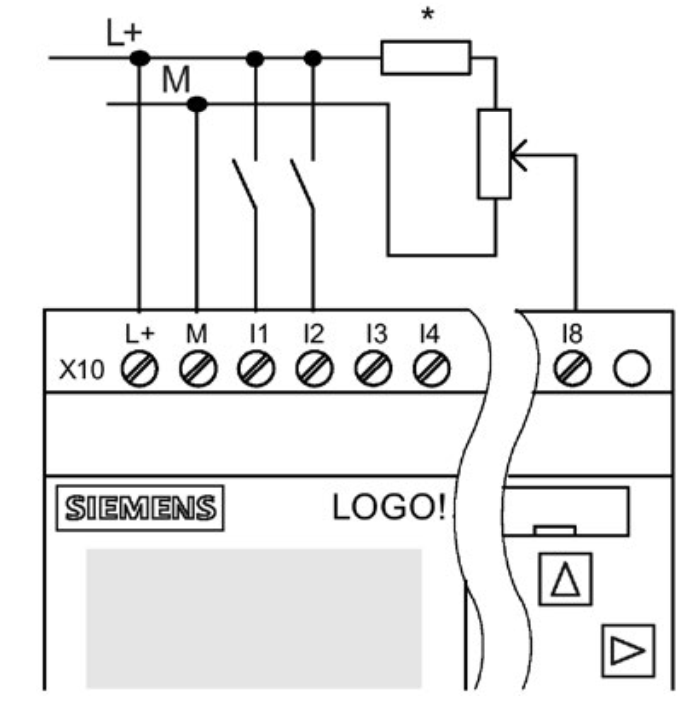
\includegraphics[width=\textwidth,height=.3\textheight,keepaspectratio]{images/cablage_alimentation_entrees.png}
    \caption{Cablage de l'alimentation et des entrées sur le module de base}
\end{figure}

\subsection{Cablage des sorties à relais}
\begin{figure}[h!]
    \centering
    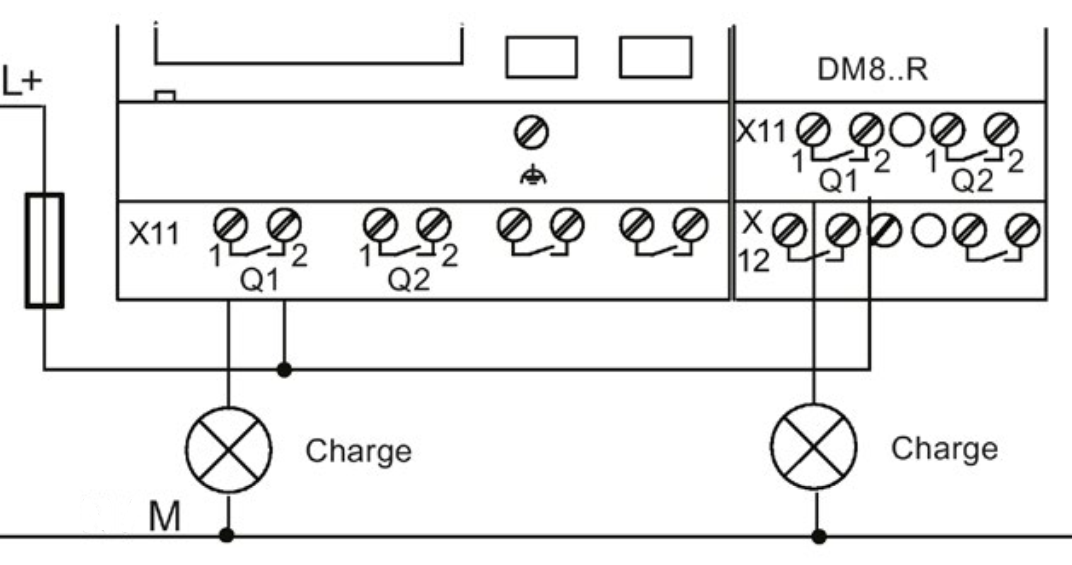
\includegraphics[width=\textwidth,height=.3\textheight,keepaspectratio]{images/cablage_sorties_relais.png}
    \caption{Cablage de l'alimentation et des entrées sur le module de base}
\end{figure}
\end{document}
